% Template for ICIP-2018 paper; to be used with:
%          spconf.sty  - ICASSP/ICIP LaTeX style file, and
%          IEEEbib.bst - IEEE bibliography style file.
% --------------------------------------------------------------------------
\documentclass{article}
\usepackage{spconf,amsmath,graphicx}

% Example definitions.
% --------------------
\def\x{{\mathbf x}}
\def\L{{\cal L}}

% Title.
% ------
\title{\fontsize{30}{40}\selectfont Traffic Sign Classifier}
%
% Single address.
% ---------------
\name{Vivin Peris(16ME221), Renu Prasad(16ME263), Shyam Santhosh(16EC244), Shravani M(16EC112)\ }
\address{National Institute of Technology Karnataka \\* Surathkal Mangalore India-575025}


%
% For example:
% ------------
%\address{School\\
%	Department\\
%	Address}
%
% Two addresses (uncomment and modify for two-address case).
% ----------------------------------------------------------
%\twoauthors
%  {A. Author-one, B. Author-two\sthanks{Thanks to XYZ agency for funding.}}
%	{School A-B\\
%	Department A-B\\
%	Address A-B}
%  {C. Author-three, D. Author-four\sthanks{The fourth author performed the work
%	while at ...}}
%	{School C-D\\
%	Department C-D\\
%	Address C-D}
%
\begin{document}
%\ninept
%
\maketitle
%
\begin{abstract}
One of the most common root cause of road accidents has been human factors. Indeed, the potentially dangerous choices made by the driver might be intentional as they might be the result tiredness, drowsiness or a poor perception and interpretation of seen scenes. The introduction of autonomous vehicles will certainly reduce these causes or even make them disappear. The work we did aims to recognising traffic signs which is one of the essential parts to the ultimate Self-Driven Car System in order to aid the decision making in a self-driving car. Here we use deep learning approach where lenets. The main project aim is to recognising the traffic signs system detects and classifies more traffic signs and attempts to develop an onboard warning camera captured colour images.
\end{abstract}
%

%
\section{Introduction}
\label{sec:intro}
Human factor remains the most common cause of road
mortality. Indeed, the potentially dangerous choices made by
the driver might be intentional (speed driving, for example) as
they might be the result of physical tiredness, drowsiness or a
poor perception and interpretation of seen scenes. The
introduction of autonomous vehicles will certainly reduce these
causes or even make them disappear.\\
As part of the development of these autonomous vehicles,
particularly driving assistance systems, several manufacturers
and laboratories have oriented their works towards the
exploitation of visual information because of its usefulness for
the detection of road, vehicles, pedestrians and traffic signs.
The principle of driving assistance systems aiming at road signs
recognition is to detect signs, interpret their meaning, then
transmit the information to the driver (by a projection on a
windshield, a screen or a smartphone) or even better, transmit
the information to the vehicle that carries out the execution
without needing a human decision. However, given that the
classical approach has been bounded by well-structured models
of traffic signs (undistorted and completely visible models)
only, it became necessary to consider real characteristics of the
road environment. For this, the current researches are moving
towards the development of recognition systems which are
more adapted to real images of road signs that do not generally
look like their models.

\section{METHODOLOGY}
\label{sec:majhead}

The proposed model is focused on the developing field of smart cars which require smart classification of the data. One of the main limitations faced were worn/damaged traffic signs cannot be classified.
Proposed System:
1. Initial step – training with sample images of traffic signs using train set
2. Images captured by cameras in cars are fed into the model for testing
3. Neural Network is built on lenet to classify and detect road traffic signs. The trained network is used in the inception model by google to further enhance the accuracy on the test set.
4. If a live feed is developed, the model will classify and display the traffic sign with its name

\subsection{Data}
\label{ssec:subhead}

The German Traffic Sign Benchmark (GTSB) consists of 43 different traffic signs with each image having 32×32 pixels in size. This dataset has 34,799 images as training data (Using these number of images we have to train a neural network) and 12,630 images as test data. Each image is a photo of one of the 43 classes of traffic signs. While going through each class images and plotting the distribution of a number of images, the following graph is obtained. Looking at the distribution, it can be deduced that some classes have less than 250 images and some of them have more than 2000. The dataset is therefore highly unbalanced. This could create a bias in the model which would be trained as a result. This is further corrected by using epochs which help to minimise any form of error

\subsection{Data preprocessing}
\label{ssec:subhead}
Grayscaling: The image from the received dataset were in RBG format, giving an additional depth to the image for training. To simplify the model as the colour of the traffic signal does not matter as much, the image was toned down to grayscale.\\
Warping: The images received in the dataset were not perfect. They were pictures taken by people from various angles and wasn’t very uniform to emulate the fact that during a real situation the camera situated in the self-driving car for the traffic sign classification may not be perfectly aligned to the sign. As a result, these pictures had to be warped to a uniform format so that the model can train on it easily and effectively.\\
Scaling: The dataset pictures were of varying resolutions and had to be scaled to a uniform scale to bring about uniformity in the model.\\
Rotation: The rotation of the image also provides us with more data to work with from which we can anticipate the same output. A rotated image of “Give Way” should be classified as the same by the classifier too.\\
Brightness: The brightness of the images was tuned to give a uniform input of images which would highlight different parts of the traffic sign. This helped the model to identify key shapes and objects that it needs to give closer attention to than the other attributes.

\subsection{Adam Optimizer}
\label{ssec:subhead}

Adam (Adaptive Moment estimation) is an adaptive learning rate method, which means, it computes individual learning rates for different parameters. Its name is derived from adaptive moment estimation, and the reason it’s called that is because Adam uses estimations of first and second moments of gradient to adapt the learning rate for each weight of the neural network.\\
N-th moment of a random variable is defined as the expected value of that variable to the power of n.\\*
\\*
m_n=E[X^n ]\\*
Where, \\*
mn = moment\\*
X = random variable\\

\noindent The gradient of the cost function of neural network can be considered a random variable, since it usually evaluated on some small random batch of data. The first moment is mean, and the second moment is un-centered variance (meaning we don’t subtract the mean during variance calculation).\\
To estimates the moments, Adam utilizes exponentially moving averages, computed on the gradient evaluated on a current mini-batch:\\*
\\*
m_t= β_1 m_(t-1)+(1-β_1 ) g_t\\*
v_t= β_2 v_(t-1)+(1-β_2)g_t^2\\*
Where \\*
m,v = moving\hspace{1.5 mm} averages,\\*
g = gradient\hspace{1.5 mm} on\hspace{1.5 mm} current mini-batch,\\*
betas = new\hspace{1.5 mm} introduced\hspace{1.5 mm} hyper-parameters\hspace{1.5 mm} of\hspace{1.5 mm} algorithm.\\


Properties of Adam:
\begin{itemize}
   \item Actual step size taken by the Adam in each iteration is approximately bounded the step size hyper-parameter. This property adds intuitive understanding to previous unintuitive learning rate hyper-parameter.   
   \item Step size of Adam update rule is invariant to the magnitude of the gradient, which helps a lot when going through areas with tiny gradients (such as saddle points or ravines). In these areas SGD struggles to quickly navigate through them.
   \item Adam was designed to combine the advantages of Adagrad, which works well with sparse gradients, and RMSprop, which works well in on-line settings. Having both of these enables us to use Adam for broader range of tasks. Adam can also be looked at as the combination of RMSprop and SGD with momentum.
\end{itemize}

% Below is an example of how to insert images. Delete the ``\vspace'' line,
% uncomment the preceding line ``\centerline...'' and replace ``imageX.ps''
% with a suitable PostScript file name.
% -------------------------------------------------------------------------
\begin{figure}[htb]

\begin{minipage}[b]{1.0\linewidth}
  \centering
  \centerline{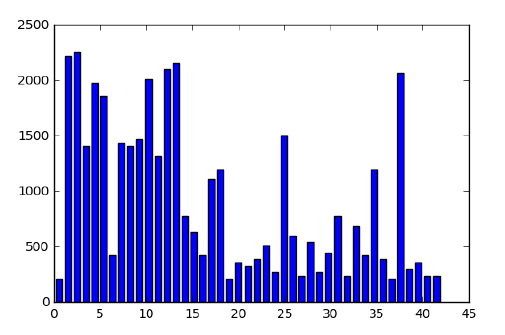
\includegraphics[width=8.5cm]{one.PNG}}
%  \vspace{2.0cm}
  \centerline{Data Classes}\medskip
\end{minipage}
%

\caption{Unbalanced class numbers}
\label{fig:res}
%

\begin{minipage}[b]{1.0\linewidth}
  \centering
  \centerline{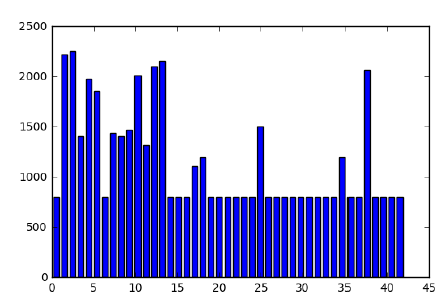
\includegraphics[width=8.5cm]{two.PNG}}
%  \vspace{2.0cm}
  \centerline{ Data Classes}\medskip
\end{minipage}
%

\caption{Balanced class numbers}
\label{fig:res}
%

\end{figure}

% To start a new column (but not a new page) and help balance the last-page
% column length use \vfill\pagebreak.
% -------------------------------------------------------------------------
%\vfill
%\pagebreak

\subsection{LeNet model architecture}
\label{ssec:subhead}

\begin{minipage}[b]{1.0\linewidth}
  \centering
  \centerline{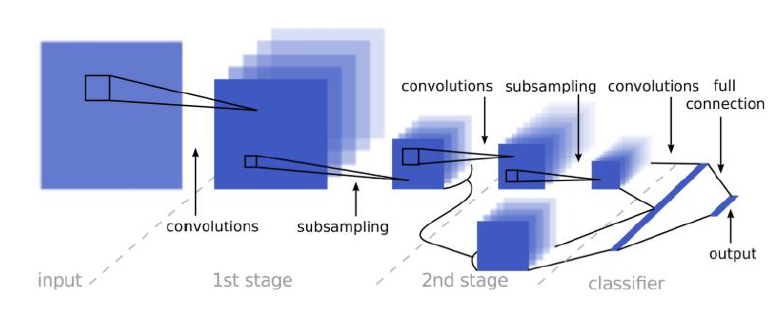
\includegraphics[width=8.5cm]{three.PNG}}
%  \vspace{2.0cm}
  \centerline{}\medskip
\end{minipage}
%
\begin{center}
\caption{\textbf{Fig. 3.} LeNet Architecture}
\label{fig:res}
\end{center}
%

\end{figure}
LeNet consists of 
\begin{itemize}
   \item 5x5 convolution (32x32x1 in, 28x28x6 out)    
   \item ReLU
   \item 2x2 max pool (28x28x6 in, 14x14x6 out)
   \item  5x5 convolution (14x14x6 in, 10x10x16 out)
   \item ReLU
   \item 2x2 max pool (10x10x16 in, 5x5x16 out)
   \item 5x5 convolution (5x5x6 in, 1x1x400 out)
   \item ReLU
   \item Flatten layers from numbers 8 (1x1x400 -> 400) and 6 (5x5x16 -> 400)
   \item Concatenate flattened layers to a single size-800 layer
   \item Dropout layer
   \item Fully connected layer (800 in, 43 out)
\end{itemize}
\subsection{Inception Network}
\label{ssec:subhead}

\begin{minipage}[b]{1.0\linewidth}
  \centering
  \centerline{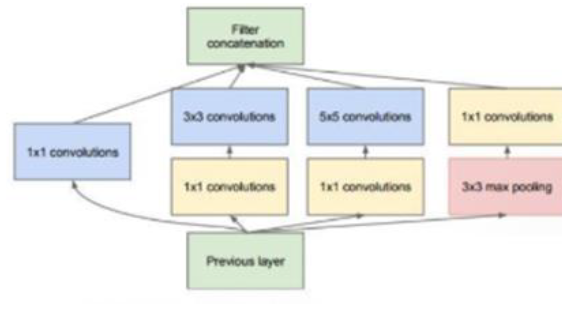
\includegraphics[width=8.5cm]{four.PNG}}
%  \vspace{2.0cm}
  \centerline{}\medskip
\end{minipage}
%
\begin{center}
\caption{\textbf{Fig. 4.}  Inception Model}
\label{fig:res}
\end{center}
%

\end{figure}

\subsection{Training Process}
\label{ssec:subhead}
The training was done on google collab GPU on the dataset. The process was initially tested on the Laptop hardware, however due to time constraints, we shifted to google collab as it was much faster to train and test the neural network

\section{RESULTS}
\label{sec:ref}
The results after successful training are:\\*
LeNet
\begin{itemize}
   \item Validation Accuracy:99.1%
   \item Test Accuracy: 95.1%
\end{itemize}
Inception Model
\begin{itemize}
   \item Validation Accuracy:98.2%
   \item Test Accuracy: 96.5%
\end{itemize}



\begin{thebibliography}{9}
\bibitem{} 
Djebbara Yasmina, Rebai Karima, Azouaoui Ouahiba,
\textit{}. 
“Traffic Signs
Recognition with Deep Learning”, 2018 International Conference on
Applied Smart Systems (ICASS'2018) – IEEE Explore
\bibitem{} 
P. Dewan, R. Vig, N. Shukla and B. K. Das,
\textit{}“An Overview of Traffic
Signs Recognition Methods,” International Journal of Computer
Applications, Vol. 168 – N..11, June 2017 
[\textit{}]. 
 
\bibitem{} 
L. Abdi,
\texttt{}
“Deep learning traffic sign detection, recognition and
augmentation,” Proceedings of the Symposium on Applied Computing,
Maroc, 2017, p. 131-136
\end{thebibliography}





\end{document}
